\documentclass[english, 11pt]{article}

\usepackage[T1]{fontenc}
\usepackage[utf8]{inputenc}
\usepackage{geometry}
\usepackage{url}
\usepackage{amsthm}
\usepackage{mathrsfs}
\usepackage{makeidx}
\usepackage{graphicx}
\usepackage{babel}
\usepackage{fancyhdr}
\usepackage[T1]{fontenc}
\usepackage{amsmath,amssymb}
\usepackage{url}
\usepackage{enumerate}
\usepackage{tikz}

\tikzstyle{na} = [shape=rectangle, inner sep =0pt]

\newcommand{\tocandfigures}{
	\rule[0.5ex]{1\columnwidth}{1pt}
	Last Revision: \today
	\noindent \begin{flushleft}
	\makeatletter
	\makeatother
	\setcounter{page}{1}
	\setcounter{secnumdepth}{0} %Hide section number in header
	\end{flushleft}
	\noindent \begin{flushleft}
	\tableofcontents{}
	\par\end{flushleft}
	\noindent \begin{flushleft}
	\rule[0.5ex]{1\columnwidth}{1pt}
	\par\end{flushleft}
	\noindent \begin{flushleft}
	\newpage{}
	\par\end{flushleft}
}


\newcommand{\thiscoursecode}{PHYS 5243}
\newcommand{\thiscoursename}{Solid State Physics}
\newcommand{\thisprof}{Sheena Murphy}
\newcommand{\me}{Chase Brown}
\newcommand{\thisterm}{Spring 2015}


% helpful stuff
\newcommand{\vect}[1]{\textrm{\textbf{#1}}}

% Headers
\pagestyle{fancy}

%%%%% TITLE %%%%%
\newcommand{\notefront} {
	\pagenumbering{roman}
	\begin{center}
		\textbf{\Huge{\thiscoursecode}}{\Huge \par}
		{\Large{\thiscoursename}}\\ \vspace{0.1in}
		\thisprof \ $\bullet$ \ \thisterm \ $\bullet$ \ University of Oklahoma \\
	  \end{center}
  }

\begin{document}
\tikzstyle{every picture}==[remember picture]
	\thispagestyle{empty}
	\notefront
	% Table of Contents and List of Figures
	\tocandfigures		

	
	\section{2015-01-09: Chapter 1 - About Condensed Matter Physics}
		\subsection{Syllabus}
		\underline{Read Chapters 1 and 2 before next lecture} \\
		Graduate Student $\rightarrow 15\%$ of the grade is HW. \\
		2 Midterms: Wednesday nights ($\sim$ 4 hours are given to do them). \\
		The Final counts for $\sim 25\%$ of grade for Graduate and Undergraduate Students. \\
		\mbox{Get the other books required for class $\rightarrow$ they are important!} \\
		Graduate Studnet difference $\rightarrow$ potentially a physics simulation will be required. \\

 		\begin{center}
			\line(1,0){425}
		\end{center} 
		\subsection{Class Notes}

		\begin{center} 
			\framebox{
				\tikz\node[na](word1){
					\thiscoursename
				};
			} \\
			(Condensed Matter Physics)
		\end{center} 

		
		\tikz\node[na](word2){Physics}; of complexity $\rightarrow$ statistical physics (thermodynamics)

		\begin{tikzpicture}[overlay]
			\path[->, black, thick](word1) edge [out=180, in=180] (word2);
		\end{tikzpicture}

		\begin{description}
			\item Collections of atoms
				\begin{description} 
					\item{Somewhat under atomic physics field}
					\item{Solids, liquids, and polymers}
				\end{description}
		\end{description}
		
		Hamiltonian:
		\begin{equation*}
				\hat{H} = \underbrace{\frac{\mathbf{p_n}^2}{2 M_n}}_{\substack{momentum\\of\\ions}} + 
							\underbrace{\frac{\mathbf{p_e}^2}{2 M_e}}_{\substack{momentum\\of\\electrons}} +
							\underbrace{\frac{e^2}{r_{i1}-r_{j1}}}_{\substack{repulsion\\between\\ions}}  + 
							\underbrace{\frac{e^2}{r_{i2}-r_{j2}}}_{\substack{repulsion\\between\\electrons}}  -
							\underbrace{\frac{e^2}{r_{i1}-r_{j2}}}_{\substack{attraction\\between\\electrons\ and\ ions}}
		\end{equation*}
		
		At the moment only $\sim$100 atoms can be solved (using supercomputer) $\rightarrow$ very difficult! \\
		\begin{description}
			\item Emergent phenomenon is common
			\begin{description}
				\item Superconductivity is emergent from collection of atoms
			\end{description}
		\end{description}
	


	\pagebreak
	\section{2015-02-20: Chapter 1 (Kittel) - Crystal Structure}
		Test on Everything but Crystal Structure.
		Closed book but will provide equations.
		\subsection{Primitive Cells}
			Crystal Structure handout.
			\begin{description}
				\item[(100)]  \ 
					plane of atoms.
				\item[$\{$100$\}$] \
					family of planes.
				\item[\ [100] ] \
					direction.
			\end{description}
			
			
	
	
	\pagebreak
	\section{2015-04-06: Chapter 8 Kittel? - Semiconductor}
		\Large{\textbf{Exam postponed until Wednesday next week}}\\
			All material will be covered up to semiconductors, no p-n junctions, but will have n and p semiconductors.
			
			\begin{description}
				\item[n-type SC] donor level lives close to conduction band.
				\item[p-type SC] donor level below valence band
			\end{description}
			
			 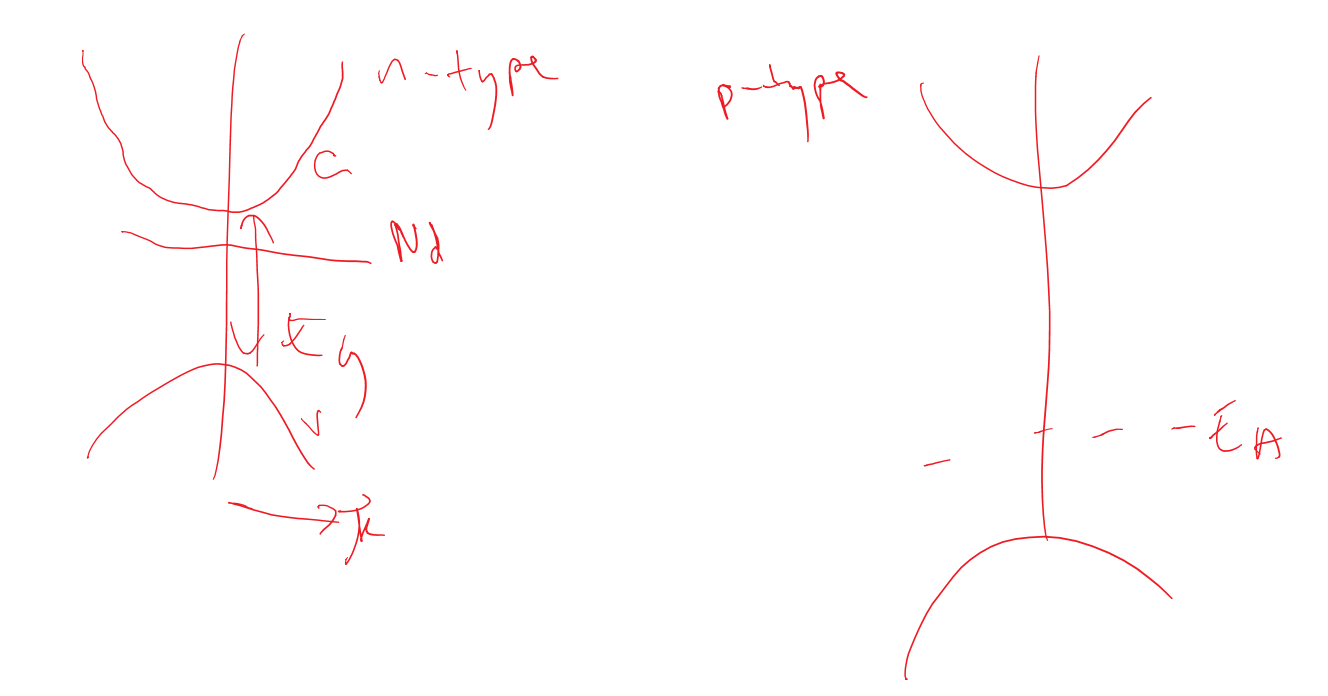
\includegraphics{pntype.png} 
			 
	\pagebreak
	\section{2015-04-08: Optical Properties of Materials -  Chapter 14 and 16 in Kittel}
		Will be doing: \\
		Superconductivity - single lecture \\
		Graphene - single lecture \\
		
		~\\
		Drude Model - fermi surface shifts in the reciprocol space due to electric field\\
		Then we talked of SdH\\
		What we haven't talked about how light interacts with material.
		~\\
		Guass's Law:
		\begin{equation}
			\nabla \cdot \vect{E} = \frac{\rho}{\epsilon_0}
		\end{equation}
		\begin{equation}
			\rho_{total} = \rho_{ext} + \rho_{int}
		\end{equation}
		$\rho_{int}$ is materials dependent
		\begin{equation}
			\vect{D} = \epsilon_0 \vect{E} + \vect{p} = \epsilon \epsilon_0 \vect{E}
		\end{equation}
		
		$\vect{D}$ is function of $\omega$ and $\vect{k}$.  
		
		\begin{enumerate}[A]
			\item $\epsilon (\omega,0)$ : $k \rightarrow 0$ ,$x \rightarrow \infty$\\
					collective excitations of Fermi sea\\
				 $\epsilon (0,k)$ : electro static response electron electron screening\\
		\end{enumerate}
		\begin{enumerate}[A]
			\item Long Wavelength Response\\
		\begin{equation}
			m\frac{d^2x}{dt^2} = -e\vect{E}
		\end{equation}
		\begin{equation}
			\vect{E}\sim E_0 e^{-i\omega t}
		\end{equation}
				\begin{equation}
			x \sim x_0 e^{-i\omega t}
		\end{equation}
				\begin{equation}
			-m\omega^2 x(t) = -e E9t)
		\end{equation}
				\begin{equation}
			x(t) = + \frac{eE(t)}{m\omega^2}
		\end{equation}
				\begin{equation}
			x_0 \frac{eE_0}{m\omega^2}
		\end{equation}
		\end{enumerate}
		dipole moment of one electron
		\begin{equation}
			\vect{p} = -e X_0
		\end{equation}
		\begin{equation}
			\vect{p}_0 = \frac{\text{ \# of dipoles}}{\text{volume}} = -e x_0 n = \frac{-e^2 n E_0}{m\omega}
		\end{equation}
		$\vect{p}_0$ is the polarization
						\begin{equation}
			\epsilon(\omega) = \frac{D(\omega)}{\epsilon_0 E(\omega)}= 1 + \frac{P(\omega)}{\epsilon E(\omega)} = 1 - \frac{2^2n}{\epsilon_0 m \omega^2}
		\end{equation}
		Plasmon frequency:
						\begin{equation}
			\omega_p^2 = \frac{n_e^2}{m\epsilon_0}
		\end{equation}
						\begin{equation}
			\epsilon(\omega) = 1 - \frac{\omega_p^2}{\omega^2}
		\end{equation}
		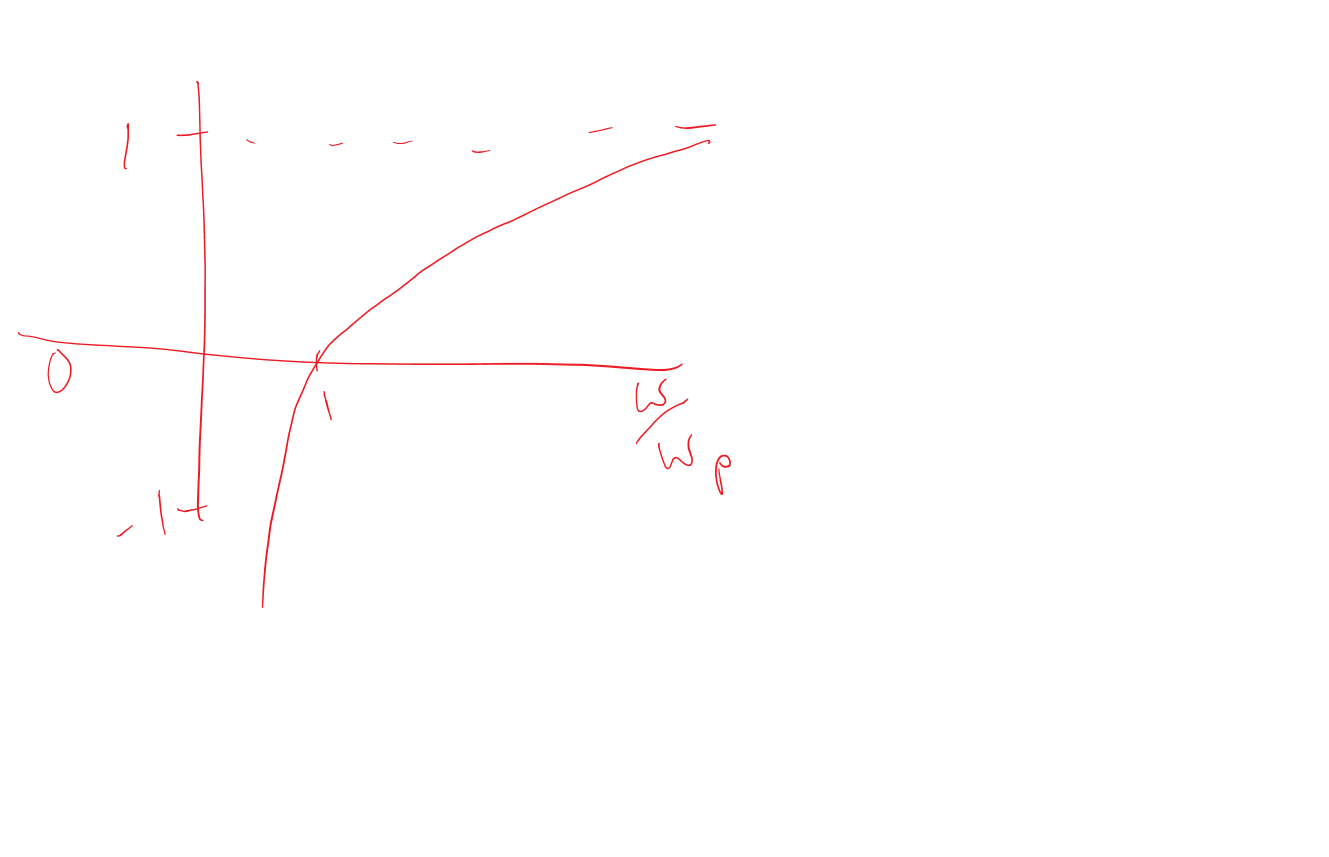
\includegraphics{plasmonfreq.png}
		
		Non magnetic:
		\begin{equation}
			\mu_0 \frac{d^2\vect{D}}{dt^2} = \nabla^2 \vect{E}
		\end{equation}
		\begin{equation}
			\vect{E} \propto e^{i\omega t} e^{i\vect{k} \cdot \vect{r}}
		\end{equation}
		\begin{equation}
			D = \epsilon (\omega, k) \vect{E}
		\end{equation}
		
		\begin{equation}
			\epsilon(\omega, \vect{k} \epsilon_0 \mu_0 \omega^2 = k^2
		\end{equation}
		
		In general:
		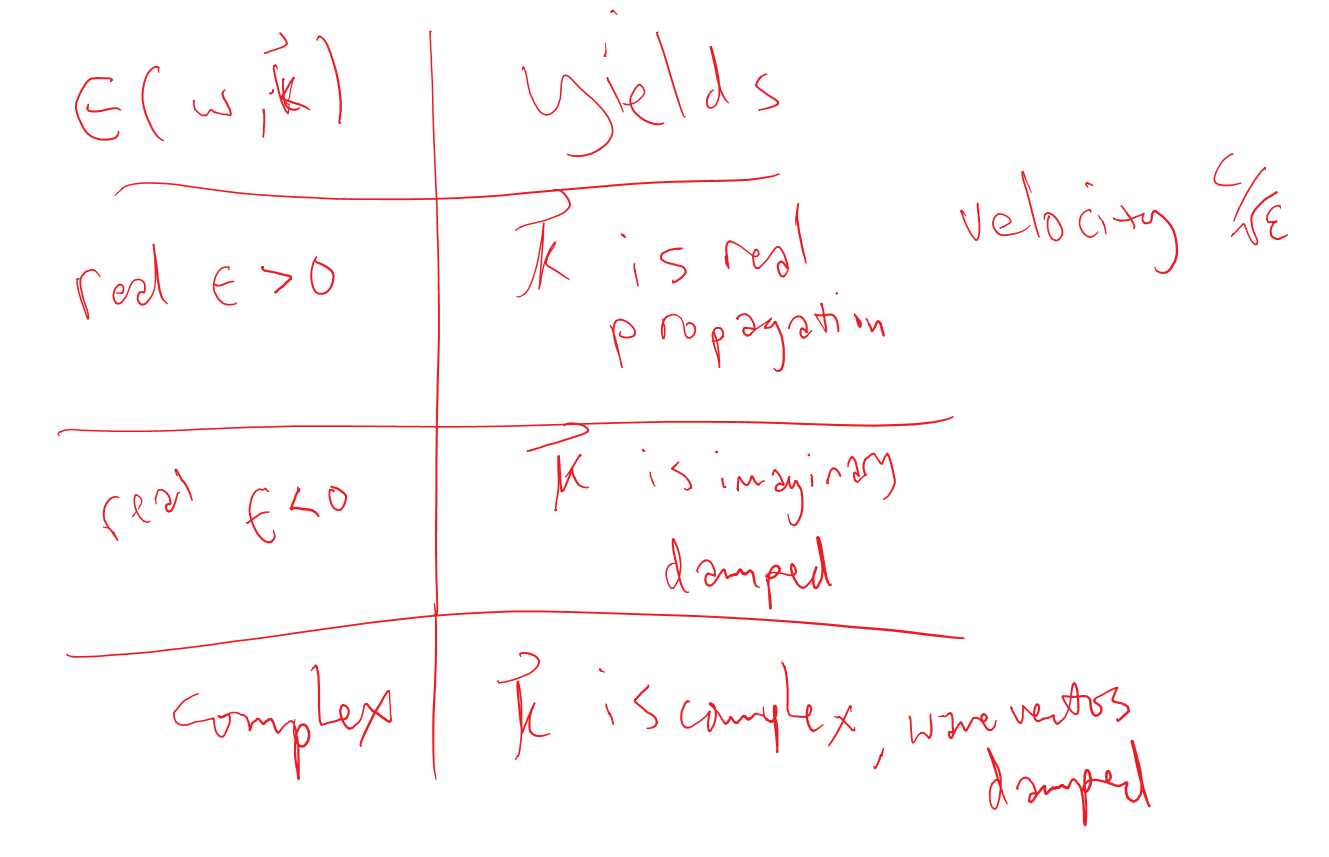
\includegraphics{table.png}
		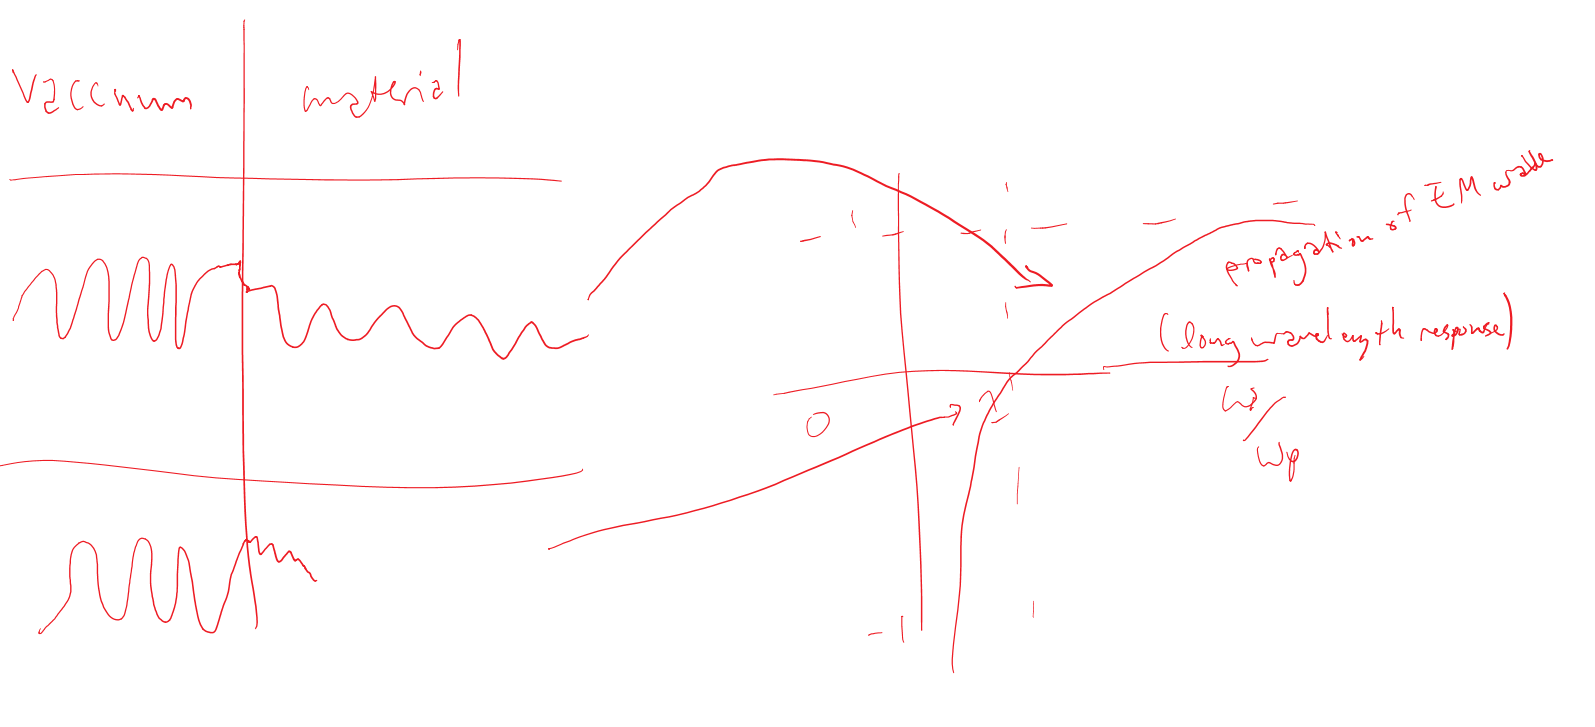
\includegraphics{waves.png}
		
		\pagebreak
		\section{2015-04-22: Tight Binding - by someone not Murphy}
			\textbf{Tight binding}
			In a s system with translational symetrry
			
			
			with $i=1...N$ lattice sites.
			
			If H is the Hamiltonian, we assume that:
			\begin{equation}
				\langle i | H | j \rangle = \begin{cases} -t & \text{for nearest neighbor} \\   0 & \text{otherwise} \end{cases}
			\end{equation}
			
			The eigenenergies are:
			\begin{equation}
				E_k = \langle k |H | k\rangle  = \frac{1}{N} \sum_{i=1}^N \sum_{j=1}^N \langle i | H | j \rangle 
			\end{equation}
			\begin{equation}
				= \frac{1}{N} \sum_{\delta}\langle i |H|j\rangle e^{ik\cdot \delta}
			\end{equation}
			
			\begin{equation}
				= -t \sum_{\delta}  e^{ik\cdot \delta}
			\end{equation}
			
			where $\delta$ are the NN vectors
			
			In a square lattice,
			$\delta = (\pm a,0),(0, \pm a)$
			
			 \begin{equation}
			 	e_k = -t \sum_\delta e^{i k \cdot \delta} = -2t[cos(k_x a) + cos(k_y a)]
			 \end{equation} 
	
	
		\textbf{Graphene}
		Unlike a square in a triangle lattices, honeycomb lattice is not a Bravais Lattice since it cannot be generated by a single set of latice generators
		The two sublattices require a component bases:
			
			\begin{equation}
				|i, S \rangle
			\end{equation}
			
			where $S=a,b$ for sublattice a or b.
			
			
			\begin{equation}
				\langle k s |H| k s' \rangle=   \frac{1}{N} \sum_{i=1}^N \sum_{j=1}^N \langle i s | H | j s \rangle  e^{-i k \cdot r}e^{i k \cdot r}
			\end{equation}
			
			\begin{equation}
				\langle k s |H| k s' \rangle =   \frac{1}{N} \sum_{i=1}^N -t (1-\delta_{s,s'}) e^{ik \cdot \delta_{s,s'}} 
			\end{equation}
			
			\begin{equation}
				\langle k a |H| k b \rangle=  -t \sum_{\delta}  e^{i k \cdot \delta_{ab}}
			\end{equation}
			
			\begin{equation}
				\langle k a |H| k b \rangle =  -t \sum_{\delta}  e^{i k \cdot \delta_{ba}}
			\end{equation}
			
			Since
			
						\begin{equation}
				\delta_{ab}^1 = (a,0)
			\end{equation}
			\begin{equation}
				\delta_{ab}^2 = (-a/2,\sqrt{3}/2a)
			\end{equation}
			\begin{equation}
				\delta_{ab}^3 = (-a/2,-\sqrt{3}/2a)
			\end{equation}
			
			\begin{equation}			
				H_k^{ab} = \langle k a |H| k b \rangle =  -t \phi_k
			\end{equation}
			\begin{equation}			
				H_k^{ba} = \langle k b |H| k a \rangle =  -t \phi_k^*
			\end{equation}
			
			where $\phi_k = \sum_\delta e^{i k\cdot \delta}$.
			
			The eigen values are 
			\begin{equation}
				E_k = \pm t |\phi_k|
			\end{equation}
			
			Expanding $\phi_k$ around H:
			
			\begin{equation}
				\phi_{k+p} = (p_x - i p_y) \frac{3}{2} a
			\end{equation}
			
			where p is the deviation from H
			
			\begin{equation}
				H_p = \nu p\cdot \sigma
			\end{equation}
			
			(DIrac equaiton)  which is why it's called a Dirac point
			
			where $\sigma = (\sigma_x, \sigma_y)$ are Pauli matrices and $\nu = \frac{3}{2}ta$ is the Fermi velocity
			
			
			
			Eigen vectors
			\begin{equation}
				\nu \sigma\cdot p \psi_\pm = \pm \nu a \psi_\pm
			\end{equation}
			
			\begin{equation}
				\psi_\pm = \frac{1}{\sqrt{2}} \begin{matrix} 1 \\ \pm e^{i \theta a} \end{matrix} e^{i \delta\cdot r}
			\end{equation}
			
			(Bloch wavefunction)
			
			\textbf{Berry Phase}
			\begin{equation}
				\gamma = \oint_c da \psi_{\pm,a}^+ \nabla_a \psi_{\pm, a}
			\end{equation}
			
			
			
\end{document}

